\chapter{Xestión do proxecto}
A xestión do proxecto ten como finalidade definir e alcanzar os obxectivos do mesmo, ó tempo que se optimiza o uso de recursos, tanto humanos como materiais.

Na sección III do PMBOK\cite{PMBOK} descríbense amplamente os distintos tipos de procesos que se inclúen dentro da xestión do proxecto, non obstante, para cada proxecto concreto será necesario seleccionar os máis apropiados para cumprir co obxectivo do mesmo.

\section{Alcance do proxecto}
Os procesos de xestión do alcance do proxecto son os encargados de asegurar que o proxecto inclúa o traballo requirido, e só o requirido, para completar o proxecto de forma satisfactoria.

\subsection{Definición do alcance}\label{subsec:DefAlcance}
O obxectivo deste proxecto é dotar ó Sistema de Información Xeográfica QGIS da capacidade de consultar fontes de datos SOS e representar os datos obtidos no contorno de mapas proporcionado pola ferramenta, de xeito que podan ser explorados e analizados polo usuario. Para acadar este obxectivo desenvolverase un \emph{plugin} para o programa QGIS, coas seguintes funcionalidades básicas:

\begin{itemize}
\item Conectarse a un servidor SOS e obter as capacidades do servizo a través da operación GetCapabilities.
\item En base ás capacidades do servidor permitir xerar unha petición de observacións, de forma sinxela, sin necesidade de coñecementos técnicos do SOS.
\item Permitir modificar a petición xerada manualmente se o usuario o desexa.
\item Obter as observacións a través da operación GetObservations.
\item Coas observacións descargadas xerar unha capa vectorial que conteña a información xeográfica, temporal e os valores das propiedades observadas.
\item Xerar gráficos en dúas dimensións cos datos da capa, tanto para ver a evolución dunha propiedade con respecto ó tempo como dunha propiedade con respecto a outra.
\item Permitir visualizar a capa co plugin \emph{TimeManager} de xeito que se podan facer animacións.
\end{itemize}

\subsubsection{Criterios de aceptación}
A aceptación do produto está condicionada a que o plugin satisfaga as funcionalidades descritas no apartado do alcance do proxecto sempre e cando ó longo do desenvolvemento do proxecto non se amose que son irrealizables nas 420 horas de traballo das que consta o Traballo de Fin de Grao. En caso de que os obxectivos iniciais resultasen demasiado ambiciosos redefiniranse os mesmos de acordo cos titores.

\subsubsection{Entregables do proxecto}\label{sss:entregables}
Entregaranse ó cliente para a súa validación os distintos incrementos resultado de cada ciclo de desenvolvemento, que consistirá no \emph{plugin} empaquetado en formato instalable para o QGIS.

Ó remate do proxecto entregarase, ademais do produto software, o código fonte correspondente, a memoria do traballo realizado e demais documentación necesaria segundo o regulamento do Traballo de Fin de Grao en Enxeñería Informática da Universidade de Santiago de Compostela \cite{ReglamentoTFG}.

\subsection{Estrutura de Descomposición do Traballo}
A Estrutura de Descomposición do Traballo (EDT) axuda a dividir o proxecto en paquetes de traballo de forma xerárquica. Dado que se empregará unha metodoloxía áxil para a xestión do proxecto (Sección \ref{sec:PlanXestion}) non é necesario detallar a EDT máis do que xa se fixo no anteproxecto, que se representa na figura \ref{fig:edt}.

\begin{figure}[hbtp]
\centering
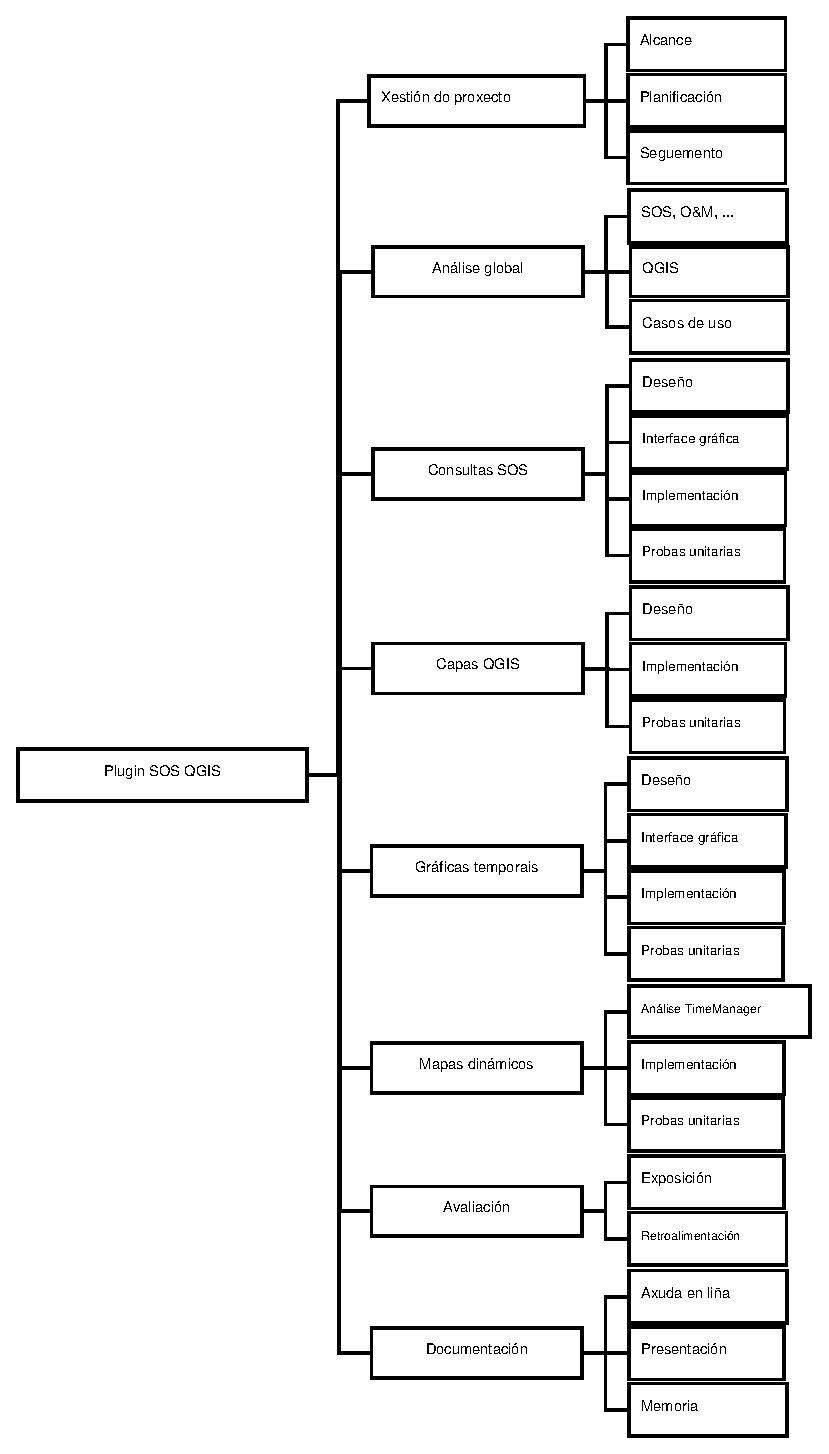
\includegraphics[height=1.0\textheight]{images/edt.eps}
\caption{Estrutura de Descomposición do Traballo}
\label{fig:edt} 
\end{figure}

\section{Metodoloxía}\label{sec:PlanXestion}
Unha das primeiras decisións a tomar á hora de iniciar un proxecto é a metodoloxía a seguir para levalo a cabo. A metodoloxía define o ciclo de vida do proxecto, e por tanto, as fases que conectan o inicio co fin do mesmo. É moi importante polo tanto que a metodoloxía elixida se adapte á natureza do proxecto, dos produtos e dos demais aspectos relacionados.

Existen dous tipos xerais de metodoloxías, as preditivas que consisten nunha planificación inicial ríxida a seguir durante todo o ciclo de vida do proxecto, e as áxiles, que asumen que existirán cambios o longo do ciclo de vida do proxecto polo que son máis flexibles para axilizar o desenvolvemento e a capacidade de adaptación ós cambios. Dada a nula experiencia previa nas tecnoloxías a empregar e  na área de coñecemento do proxecto o uso dunha metodoloxía preditiva non é aconsellable. Entre as metodoloxías áxiles seleccionase \emph{Scrum}\cite{ScrumManager}, por ser unha das máis utilizadas e porque o equipo de desenvolvemento xa está familiarizado con ela.

\subsection{Aplicación da metodoloxía Scrum}

So se aplicarán os conceptos da metodoloxía de xestión de proxectos \emph{Scrum} que resulten beneficiosos para este traballo concreto, pois debido as particularidades que presenta, ó tratarse dun equipo de desenvolvemento de unha soa persoa, e realizarse no entorno dun Traballo de Fin de Grao, algúns dos conceptos son dificilmente aplicables ou inútiles. Así pois, a continuación descríbense brevemente os conceptos dos que si se fará uso:
\begin{description}
\item[Historia de usuario ou \emph{User history}:] Representación dun requisito funcional do software mediante unha breve descrición textual. Debe ser o suficientemente sinxela como para poder estimar o tempo necesario para completala.
\item[Pila do produto ou \emph{Product Backlog}:] Lista ordenada de historias de usuario que compoñen o proxecto.
\item[Sprint:] É o período de tempo durante o cal se leva a cabo o traballo, xeralmente de 2 a 4 semanas. Cada sprint produce un incremento software, é dicir, unha nova versión potencialmente entregable.
\item[Pila do sprint ou \emph{Sprint Backlog}:] É o subconxunto de historias de usuario que serán acometidas nun sprint. Xeralmente as historias divídense en tarefas cando pasan á pila do sprint. Esta pila, así como os requisitos incluídos na mesma non poden modificarse mentres dure o sprint.
\end{description}

Na figura \ref{fig:scrum} móstrase graficamente o ciclo de vida da metodoloxía \emph{Scrum}.
\begin{figure}[hbtp]
  \centering
  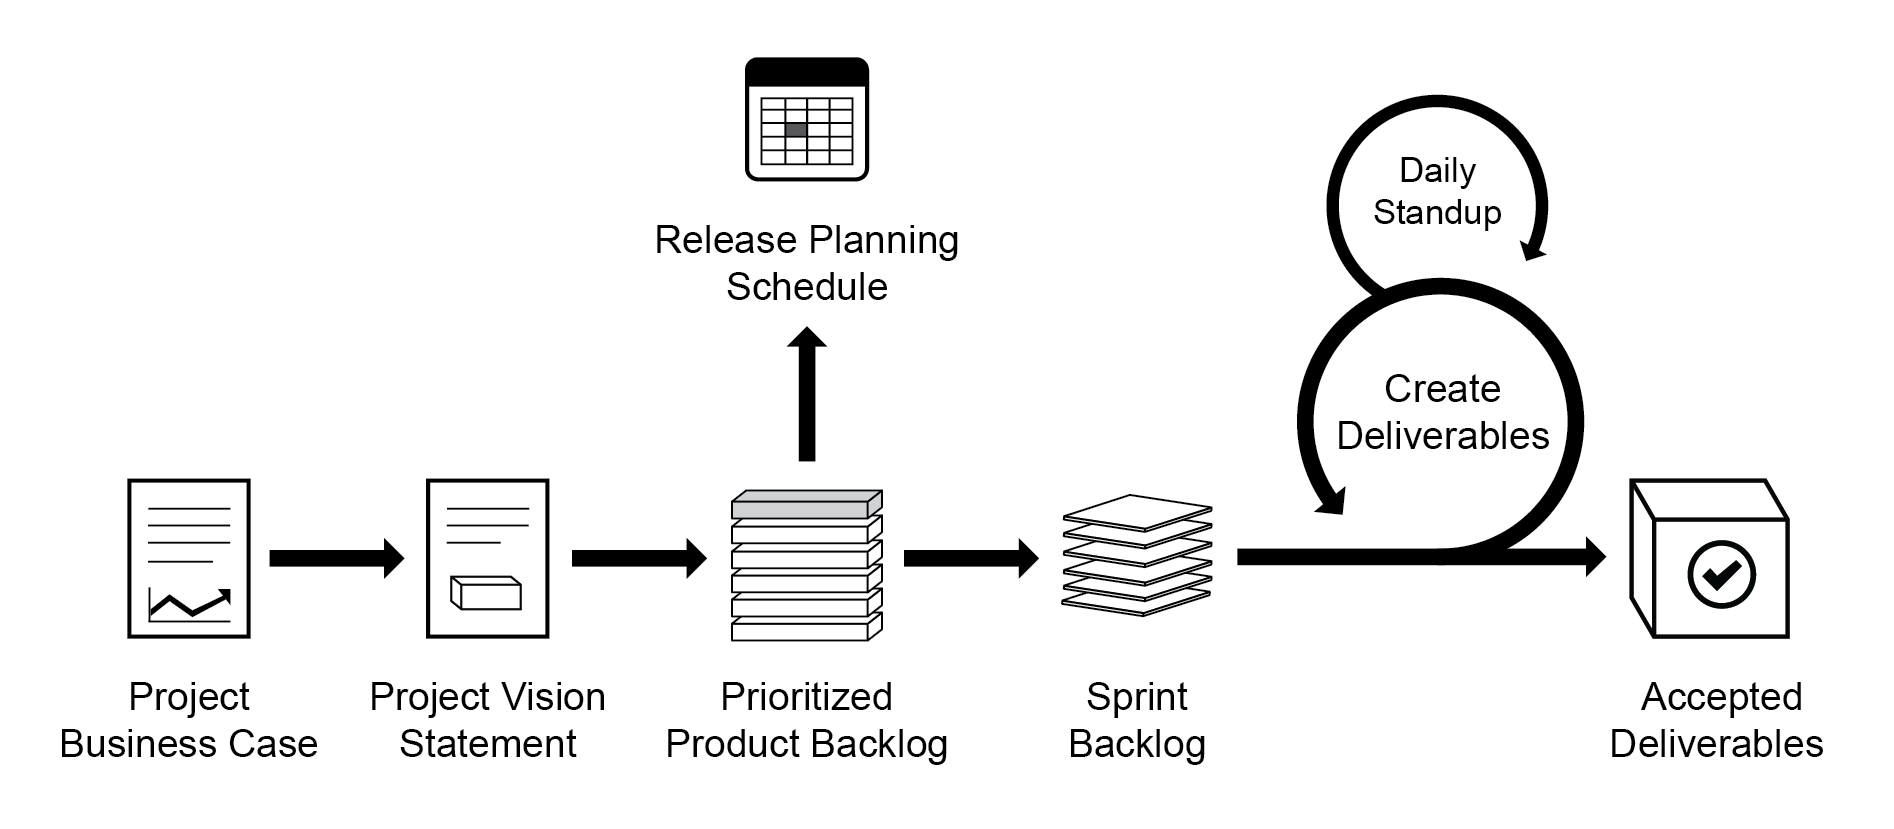
\includegraphics[width=1.0\textwidth]{images/Scrum.png}
  \caption{Ciclo da metodoloxía Scrum}
  \label{fig:scrum}
  \captionsetup{font={scriptsize,it}}
  \caption*{Fonte: \url{https://commons.wikimedia.org/wiki/File:Scrum_Flow_for_one_Sprint.png}}
\end{figure}

\section{Xestión do tempo}
A xestión do tempo do proxecto inclúe os procesos necesarios para lograr a conclusión do proxecto a tempo.

\subsection{Planificación temporal}
Tendo en conta que na metodoloxía \emph{Scrum} non se planifica inicialmente a duración nin o contido de cada sprint debemos considerar esta planificación como unha guía a seguir para organizar o traballo cronoloxicamente, non como unha planificación estrita e vinculante para o desenvolvemento do proxecto.

Para levar a cabo a planificación do proxecto faise unha revisión xeral das distintas fases, tomando como base a Estrutura de Descomposición do Traballo da figura \ref{fig:edt}. Existen diferencias significativas entre a \emph{EDT} e o diagrama de \emph{Gantt} (Figura \ref{fig:gantt}) debido a que no primeiro móstranse os paquetes de traballo necesarios para acadar os obxectivos do proxecto, mentres que no segundo se organizan cronoloxicamente as tarefas necesarias para completar ditos paquetes de traballo.

En canto ás estimacións temporais, considérase unha xornada semanal de 35 horas, que, por simplicidade, se visualiza no \emph{Gantt} como 5 horas diarias os 7 días a semana. En realidade esta dedicación será variable diariamente dependo das obrigas laborais dos membros do equipo pero co compromiso de cumprir a planificación semanalmente.

\begin{sidewaysfigure}
\centering
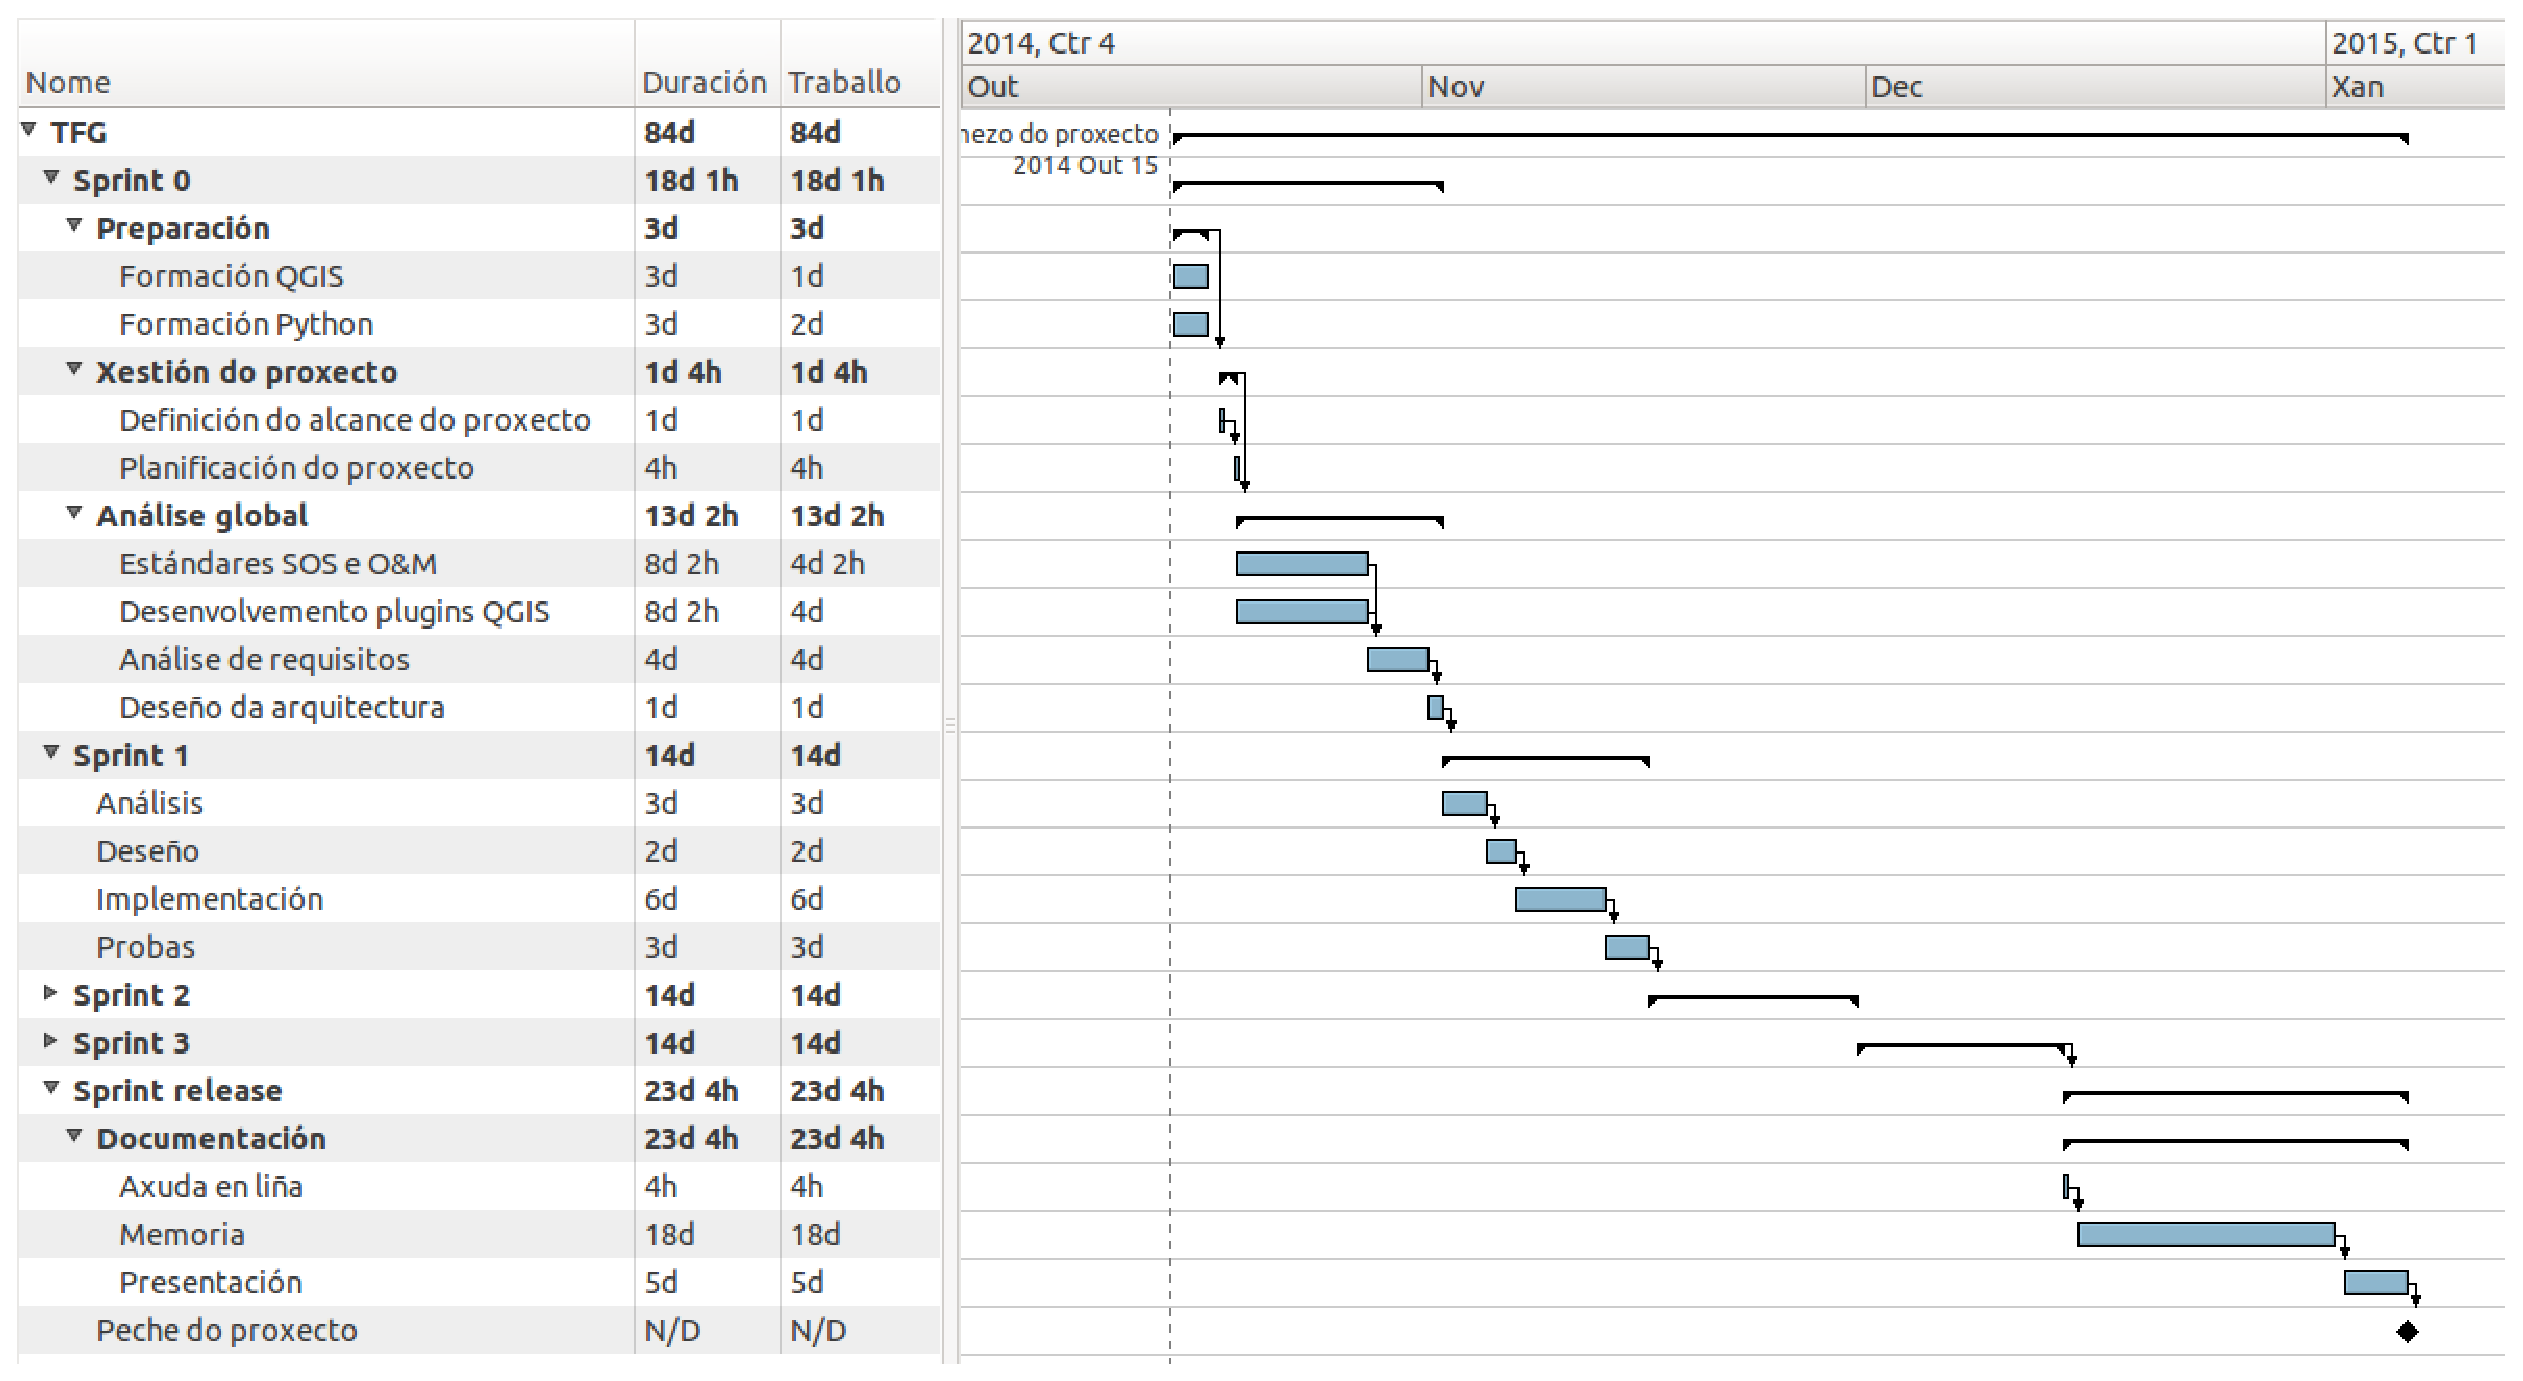
\includegraphics[width=1.0\textwidth]{images/gantt.eps}
\caption{Diagrama de Gantt}
\label{fig:gantt}
\end{sidewaysfigure}

Planificase o desenvolvemento do proxecto en cinco sprints, o \emph{Sprint 0} inicial, tres sprints normais de 70 horas e o \emph{Sprint release} final.

\subsection{Sprint 0}
Este sprint é o inicial do proxecto. É un sprint especial, pois non xerará ningún incremento, senón que se levarán a cabo os distintos procesos de iniciación do proxecto.

\subsubsection{Preparación}
\textit{15 horas}

Capacitación do equipos nas tecnoloxías empregadas no proxecto e iniciación na area de coñecemento dos Sistemas de Información Xeográfica.
Tamén se configura o entorno de desenvolvemento integrado \emph{Eclipse} co \emph{plugin} \emph{PyDev}.

\subsubsection{Xestión do proxecto}
\textit{9 horas}

Definición do alcance do proxecto, metodoloxía, xestión de custos, riscos e da configuración, e planificación do mesmo. Para realizar esta planificación é necesario crear a versión inicial da pila do produto (cadro \ref{tab:productBacklog}).

\begin{table}
\centering
\begin{tabularx}{\textwidth}{rXc} \toprule
	\# & Historia de usuario & Horas \\
	\midrule
	1 & Conexión con servidor SOS & 25 \\
	2 & Procesamento do xml de capacidades do servizo & 30 \\
	3 & Xeración de peticións básicas & 15 \\
	4 & Xeración de peticións con filtros complexos & 20 \\
	5 & Creación de peticións personalizadas & 5 \\
	6 & Xeración dunha capa vectorial a partir dos datos de observacións & 35\\
	7 & Xeración dunha capa válida para o \emph{plugin} \emph{TimeManager} & 10\\
	8 & Visualización gráfica de propiedades respecto ó tempo & 20\\
	9 & Visualización gráfica de unha propiedade con respecto a outra & 25\\
	10 & Visualización de varias series de observacións simultaneamente & 25\\
	\bottomrule
\end{tabularx}
\caption{Pila inicial do produto}
\label{tab:productBacklog}
\end{table}

\subsubsection{Análise global}
\textit{69 horas}

Realizase o estudio do estándar SOS e outros relacionados (Observations\&Measurements e SensorML) e realizase o estudio da API de QGIS\cite{APIQGIS} para a programación de \emph{plugins} en \emph{Python} e demais documentación dispoñible\cite{PyQGIS}.

Tamén se leva a cabo nesta fase a análise de requisitos e casos de uso, así como o deseño preliminar da arquitectura do software a desenvolver.

\subsection{Sprints 1, 2 e 3}
Estes 3 sprints forman a fase de desenvolvemento do proxecto, durante a que se codifican os distintos compoñentes que conforman o sistema. Cada un dos sprints ten unha duración de 70 horas de horas de traballo (2 semanas).

En cada iteración realizaranse as etapas de análise, deseño, implementación e probas para as historias seleccionadas. A previsión de historias a incluír en cada sprint é a que se mostra no cadro \ref{tab:previsionSprints}. É importante destacar que esta división das tarefas nos distintos sprints é preliminar e susceptible de ser revisada e modificada o longo das distintas planificacións do sprint que se realizan durante a execución do proxecto, cando o coñecemento do problema a resolver sexa máis profundo e polo tanto a estimación máis precisa.

\begin{table}
\centering
\begin{tabularx}{\textwidth}{rXc} \toprule
	\# & Historia de usuario & Horas \\
	\midrule
	\multicolumn{3}{c}{\textbf{Sprint 1}} \\
	1 & Conexión con servidor SOS & 25 \\
	2 & Procesamento do xml de capacidades do servizo & 30 \\
	3 & Xeración de peticións básicas & 15 \\
	\multicolumn{3}{c}{\textbf{Sprint 2}} \\
	5 & Creación de peticións personalizadas & 5 \\
	6 & Xeración dunha capa vectorial a partir dos datos de observacións & 35\\
	7 & Xeración dunha capa válida para o \emph{plugin} \emph{TimeManager} & 10\\
	8 & Visualización gráfica de propiedades respecto ó tempo & 20\\
	\multicolumn{3}{c}{\textbf{Sprint 3}} \\
	4 & Xeración de peticións con filtros complexos & 20 \\
	9 & Visualización gráfica de unha propiedade con respecto a outra & 25\\
	10 & Visualización de varias series de observacións simultaneamente & 25\\
	\bottomrule
\end{tabularx}
\caption{Previsión de historias a incluír en cada sprint}
\label{tab:previsionSprints}
\end{table}

\subsection{Sprint release}
\textit{119 horas}

Este sprint tamén e especial, pois está adicado a levar a cabo os procesos de documentación e peche do proxecto. As tarefas a desenvolver son a redacción da axuda, da memoria e da presentación para a exposición do proxecto, e a preparación de todos os entregables necesarios (ver páxina \pageref{sss:entregables}).

\section{Xestión do custo}
Debido a que este proxecto é un Traballo de Fin de Grao os custos manexados son teóricos e non se considerarán os custos indirectos (electricidade, internet e similares) ou gastos de desprazamento. A xestión de custos faise co único obxectivo de dar unha valoración económica realista do traballo realizado polo que se contemplarán os recursos humanos, os recursos materiais e os recursos software necesarios para a execución do proxecto.

\subsection{Custo de recursos humanos}
O equipo de desenvolvemento para a realización do proxecto consta dunha soa persoa, que realizará as distintas tarefas de análise, programación e documentación do mesmo. Os dous titores do proxecto non se consideran parte do equipo ó nivel de xestión de custos pois a este efecto actúan no rol de clientes.

Consideraremos como salario bruto anual para o recurso 24.000 \euro, que é segundo tecnoempleo.com\cite{InformeSalarios} o salario bruto medio para un analista/programador. Ó salario bruto débense engadir os custos do mesmo para a empresa, que tomando como referencia os datos da Seguridade Social\cite{TabCotizacion} suporía un 29,9\% do mesmo. Para o cálculo do custo por hora considerase a xornada máxima indicada no Convenio Colectivo\cite{BOEConvenio}, que son 1.800 horas de traballo ó ano.

O custo de recursos humanos é por tanto de 17,32 \euro/hora.

\subsection{Custo de recursos materiais}
Para o desenvolvemento do proxecto é necesario un ordenador capaz de executar QGIS e o IDE Eclipse. QGIS non especifica formalmente uns requirimentos mínimos e é capaz de funcionar de xeito fluído nun ordenador de gama media que se pode adquirir por uns 600 \euro. Considerando unha porcentaxe de amortización anual do 25\%, como indica a Lei 27/2014\cite{Lei27/14}, pódense imputar como custes 12,50 \euro/mes. A estes efectos deben computarse os meses naturais de duración do proxecto.

Os materiais funxibles necesarios para a realización do proxecto e os gastos de impresión e CDs para a presentación do mesmo supoñen un custe de 140 \euro.

\subsection{Custo de recursos software}
Todas as ferramentas software empregadas para a realización deste proxecto son de uso gratuíto.

\subsection{Presuposto}
No cadro \ref{tab:presuposto} amosase o resumo dos custos do proxecto, que suman un total de 7489,40 \euro.
\begin{table}[H]
\centering
\begin{tabularx}{\textwidth}{Xrrr} \toprule
	Concepto & Cantidade & Custo unitario & Total \\
	\midrule
	Custos de persoal & 420 horas & 17,32 \euro & 7274,40 \euro \\
	Amortización do ordenador & 6 meses & 12,50 \euro & 75,00 \euro \\
	Custos doutros materiais & 1 & 140,00 \euro & 140,00 \euro \\
	\midrule
	\multicolumn{3}{r}{\textbf{Total}} & \textbf{7489,40 \euro} \\
	\bottomrule
\end{tabularx}
\caption{Custos totais}
\label{tab:presuposto}
\end{table}

\section{Xestión de riscos}
A xestión de riscos ten como finalidade aumentar a probabilidade e o impacto de eventos positivos e diminuír a probabilidade e impacto dos eventos adversos para o proxecto. Implica, polo tanto, prever e xestionar os eventos que poden influír na planificación temporal, no esforzo ou no custo do proxecto ou na calidade do produto e tomar as accións necesarias para evitalos ou minimizar o seu impacto. Os catro pasos básicos a seguir para levar a cabo a xestión de riscos son:
\begin{itemize}
\item Identificación
\item Análise e catalogación
\item Planificación da resposta
\item Seguimento e control
\end{itemize}

Para catalogar os riscos en base a súa relevancia empréganse tres medidores: a probabilidade de que ocorra, o impacto que supón sobre o tempo ou esforzo, e o nivel de exposición, que é unha combinación dos valores de probabilidade e impacto. Os distintos valores para estes medidores recóllense no cadro \ref{tab:exposicion}.

\begin{table}
\centering
\begin{tabular}{@{}ccccc@{}}
\cmidrule(l){3-5}
\multicolumn{2}{c}{\multirow{2}{*}{}}                                                                       & \multicolumn{3}{c}{Probabilidade}                                                                                                                                                                                    \\ \cmidrule(l){3-5} 
\multicolumn{2}{c}{}                                                                                        & \begin{tabular}[c]{@{}c@{}}Case seguro\\ $\geq$80\%\end{tabular} & \begin{tabular}[c]{@{}c@{}}Moi probable\\ \textless80\% e \textgreater30\%\end{tabular} & \begin{tabular}[c]{@{}c@{}}Pouco probable\\ $\leq$30\%\end{tabular} \\ \midrule
\multirow{6}{*}{\rotatebox{90}{Impacto}} & \begin{tabular}[c]{@{}c@{}}Alto\\ $\geq$20\%\end{tabular}                & Alto                                                             & Alto                                                                             & Medio                                                          \\
                         & \begin{tabular}[c]{@{}c@{}}Medio\\ \textless20\% e \textgreater10\%\end{tabular} & Alto                                                             & Medio                                                                            & Baixo                                                          \\
                         & \begin{tabular}[c]{@{}c@{}}Baixo\\ $\leq$10\%\end{tabular}                   & Medio                                                            & Baixo                                                                            & Baixo                                                          \\ \bottomrule
\end{tabular}
\caption{Nivel de exposición dun risco en base a Probabilidade e Impacto}
\label{tab:exposicion}
\end{table}

\subsection{Especificación de riscos}
Co obxectivo de non engadir complexidade ó seguimento do proxecto so se planifican os riscos adversos con un nivel de exposición alto, é dicir, os riscos que é bastante probable que ocorran e que teñen un impacto negativo considerable sobre o desenvolvemento do proxecto. Para desenvolver respostas efectivas ós riscos é de moita utilidade agrupalos por causas comúns, neste caso clasificándoo en base á fonte do risco.

\subsubsection{Riscos técnicos}
\risktable	{R.TEC.01}{Complexidade do estándar SOS} %Id, Nome
			 %Descrición
		  	{O nivel de madurez e uso do estándar SOS fai que sexa un estándar extremadamente amplo e con un alto grao de liberdade. Non existe ningunha implementación que cubra o estándar na súa totalidade.}
			{Moi probable} %Probabilidade
			{Alto} %Impacto
			{Alto} %Nivel de exposición
			%Resposta
			{Só se comprometerá como imprescindible soportar as operacións básicas para obter os datos de observacións provistos pola implementación SOS realizada polo CiTIUS.}

\risktable	{R.TEC.02}{Escaseza de servidores SOS} %Id, Nome
			 %Descrición
		  	{Existen moi poucos servidores que implementen SOS abertos ó público cos que poder validar a implementación realizada.}
			{Case seguro} %Probabilidade
			{Medio} %Impacto
			{Alto} %Nivel de exposición
			%Resposta
			{Instalar en local un servidor SOS para poder probar a aplicación, e solicitar acceso ós xestionados polo CiTIUS.}
			
\subsubsection{Riscos externos}
\risktable	{R.EXT.01}{Soporte de SOS en QGIS} %Id, Nome
			 %Descrición
		  	{Implementación nativa dentro do QGIS do soporte para SOS ou a publicación de algún plugin que implemente dito soporte.}
			{Moi probable} %Probabilidade
			{Alto} %Impacto
			{Alto} %Nivel de exposición
			%Resposta
			{Reorientar o proxecto para centralo en dotar o QGIS de ferramentas específicas para interacción cos datos de sensores, sempre e cando a solución SOS implantada de soporte a implementación realizada polo CiTIUS.}

\subsubsection{Riscos de persoal}
\risktable	{R.PER.01}{Descoñecemento da ferramenta QGIS} %Id, Nome
			 %Descrición
		  	{O equipo de desenvolvemento non ten experiencia no manexo da ferramenta QGIS nin outras ferramentas de información xeográfica.}
			{Case seguro} %Probabilidade
			{Medio} %Impacto
			{Alto} %Nivel de exposición
			%Resposta
			{No plan de traballo do proxecto inclúese capacitación na ferramenta QGIS así como nos conceptos básicos sobre sistemas de información xeográfica.}

\risktable	{R.PER.02}{Descoñecemento da linguaxe Python} %Id, Nome
			 %Descrición
		  	{O equipo de desenvolvemento non ten experiencia na linguaxe de programación Python.}
			{Case seguro} %Probabilidade
			{Alto} %Impacto
			{Alto} %Nivel de exposición
			%Resposta
			{No plan de traballo do proxecto inclúese capacitación na linguaxe de programación Python.}
			
\risktable	{R.PER.03}{Situación persoal dos membros do equipo} %Id, Nome
			 %Descrición
		  	{Cambios na situación persoal ou laboral nos membros do equipo que impidan levar a cabo a dedicación estimada.}
			{Case seguro} %Probabilidade
			{Alto} %Impacto
			{Alto} %Nivel de exposición
			%Resposta
			{Volver a planificar os prazos de execución do proxecto.}
			
\subsubsection{Riscos na xestión do proxecto}
\risktable	{R.XES.01}{Error na estimación temporal} %Id, Nome
			 %Descrición
		  	{A estimación temporal inicial para a execución das tarefas é pouco precisa a causa da inexperiencia en proxectos similares.}
			{Case seguro} %Probabilidade
			{Medio} %Impacto
			{Alto} %Nivel de exposición
			%Resposta
			{A estimación inicial realizase de forma pesimista. A metodoloxía \emph{Scrum} minimiza o impacto ó permitir a refinación de requisitos e estimacións o longo do proxecto.}

\section{Xestión da configuración}
A xestión da configuración\cite{GPGC} ten como propósito establecer e manter a integridade dos elementos de traballo. No proxecto que nos ocupa os elementos de traballo a xestionar son o código fonte do \emph{plugin}, o código fonte da documentación, e os distintos entregables xerados.

\subsection{Control do código fonte}
Dentro do código fonte a xestionar inclúese tanto o código do aplicación, imaxes, documentos de axuda e demais que se inclúen no \emph{plugin} empaquetado, como o código fonte para xerar a documentación.

En ambos casos o procedemento de xestión da configuración se fai a través do sistema de xestión de versións \emph{Git}. Mantéñense en local dous repositorios diferentes, un para aplicación e outro para documentación, cada un coa súa réplica remota correspondente aloxada en \emph{GitHub}\footnote{\url{https://github.com/}}. As carpetas dos repositorios locais replícanse en \emph{Dropbox}\footnote{\url{https://www.dropbox.com/}} co obxectivo de ter unha copia redundante na nube e acceso desde distintos ordenadores en todo momento.

O método de traballo consiste en realizar un \emph{Commit} local cada vez que se remata unha tarefa e realizar un \emph{Push} ó servidor remoto cada vez que se remata unha versión susceptible de ser publicada. Deste xeito no repositorio público sempre hai unha versión estable do produto.

\subsection{Control dos entregables}
Os distintos obxectos entregables xerados o longo do proxecto, dende o anteproxecto ata a presentación do mesmo son arquivados tanto en local como na carpeta de \emph{Dropbox}. Non se realiza máis control de versións sobre os produtos entregables que o propio control realizado por \emph{Dropbox}. Esta ferramenta permite o acceso ás distintas versións gardadas de calquera tipo de ficheiro.

O servizo \emph{Dropbox} tamén permite a creación de carpetas públicas. Esta funcionalidade permítenos crear un repositorio público para QGIS no que aloxar o \emph{plugin} empaquetado de xeito que sexa moi sinxelo de instalar.